% Modle pour rapport de Stage de Fin d'Etudes de UTC
% version 0.1
% 2012-07-12
% par ZHU Yinan (zhuyinan1988@gmail.com)

\documentclass[12pt,oneside,a4paper]{book}
%Chargement des packages
\usepackage[utf8]{inputenc} % l'encodage des fichiers est utf-8, mettre [latin1] si necessaire
\usepackage[french]{babel} %le rapport est en français 
\usepackage{amsmath}
\usepackage{amsfonts}
\usepackage{amssymb}
\usepackage{graphicx} %pour afficher des images
\usepackage{float}	%pour forcer le placement des images.
\usepackage{geometry} %pour la modification des marges
\usepackage{fancyhdr} %pour modification des pieds de page
\usepackage{longtable}
\usepackage{listings}
\usepackage{subfigure}
%\usepackage[Sonny]{fncychap}
\usepackage{hyperref} %pour que les références soient des liens hypertextes
\usepackage[usenames,dvipsnames]{color} % pour les textes en gris
\hypersetup{backref, pdfborder=0 0 0}
\usepackage{ragged2e}



% Comment utiliser : 
% - la page de titre est à personnaliser (title/title.tex)
% - le contenu est à rédiger dans le répertoire pages/, s'inspirer des exemples présents dans ce modèle.
% - les annexes sont à rédiger dans le répertoire appendix/
% - la bibliographie utilise BibTex (fichier biblio.bib)
% - les variables suivantes sont à remplir :
\newcommand{\TitreRapport}{Rapport de stage TN10}
\newcommand{\DateRapport}{2012}
\newcommand{\AuteurRapport}{Yinan ZHU}
\newcommand{\NomEntreprise}{Data Gest}

%définition des marges
\geometry{hmargin=2.5cm, vmargin=2.5cm } 

%utilisation des puces anglaises.
%attention, il faut avoir une version récente de frenchb.ldf. 
\frenchbsetup{StandardItemLabels}

%Définition des en-têtes et pieds de page
\renewcommand{\headrulewidth}{0.5pt}
\renewcommand{\footrulewidth}{0.5pt}
%\fancyhead[C]{ \textcolor{Gray}{\small\TitreRapport}}
\fancyfoot[LE, RO]{ \textcolor{Gray}{ \small\AuteurRapport ~~ \vline ~~ UTC ~~ \vline ~~ \DateRapport }}

\fancyfoot[C]{\thepage}
\fancyfoot[RE, LO]{
\includegraphics[width=1.8cm]{style/images/logo_utc.png}}
%\fancyhead[LE,RO]{\thepage}
\fancyhead[LO]{\rightmark}
\fancyhead[RE]{\leftmark}


%\fancyhead[L,R]{}


% définition du tire, de la date et de l'auteur du document
\title{\TitreRapport}
\date{\DateRapport}
\author{\AuteurRapport}

\makeatletter
\newcommand{\HRule}{\rule{\linewidth}{2.5mm}}
\renewcommand\maketitle{
  \begin{titlepage}
    \begin{center}
      
\includegraphics[width=7.2cm]{title/images/logo_utc.png}
      \hspace{\stretch{1}}
      %
\includegraphics[width=5.2cm]{title/images/data-gest.jpg}

      \vspace{\stretch{0.5}}

      \begin{tabular*}{1.0\textwidth}{l @{\extracolsep{\fill}} r}
        Université de téchnologie de Compiègne \\ 			%	& \NomEntreprise 				\\
        UTC \@date 							%& La Plaine de Saint Dennis 		\\
      \end{tabular*}

      \vspace{\stretch{1.5}}
      % Title
      \begin{flushright}
        {\huge \bfseries \@title\\}
        \HRule \\[0.5cm]
        {\Large \it Rapport Final de Stage de Fin d'études \\[3.5cm]}
      \end{flushright}
      %{\large \it \@author\\}
      \begin{minipage}{1\textwidth}
        \begin{flushright} \large

          \@author \\
          Système Réseaux Informatique  \\[7.5cm]
        \end{flushright}
        \begin{flushleft}
          \emph{Tutrise:} Mme.~Angélique \textsc{Ruton} \\
          \emph{Suiveur UTC:} M.~Boris \textsc{Vidolov} \\
          \emph{Entreprise:} DATA-GEST  \\

        \end{flushleft}
      \end{minipage}
      \vspace{\stretch{2}}
      %
\includegraphics[width=1.0\textwidth]{title/images/logo_illustration.png}
      \vspace{\stretch{2}}


    \end{center}\par

  \end{titlepage}
  \setcounter{footnote}{0}

%  \global\let\thanks\relax
%  \global\let\maketitle\relax
%  \global\let\@thanks\@empty
%  \global\let\@author\@empty
%  \global\let\@date\@empty
%  \global\let\@title\@empty
%  \global\let\title\relax
%  \global\let\author\relax
%  \global\let\date\relax
%  \global\let\and\relax
}


\makeatother


\begin{document}
\pagestyle{fancy}
\maketitle
\frontmatter
\chapter{Remerciements}
%\renewcommand{\baselinestretch}{3.5}
\setlength{\parskip}{0.5\baselineskip}

%Tout d'abord, je dois remercier à ma tutrice, Angélique RUTON, elle m'a donné beaucoup d'avis dans la domaine de programmation, et aussi dans la partie de conception. En plus, j'ai approfondi aussi dans la gestion de projet. Non seulement elle m'a donné suggestions dans la partie technique, mais aussi dans m'a donné les suggestions pour mon  carrier futur duquel j'ai tiré de grands profits.  

%Ensuite, je dois remercier à mon collègue, Edouard KOMBO, qui est très chaleureux et humoristique. Il m'a  aidé souvent si j'ai eu les problème dans la programmation. En plus, il m'a donné un coup de main afin que je peux pré-embauche chez DATA-GEST


\paragraph{}
Mes remerciements s’adressent en premier lieu à ma tutrice de stage,  Madame Angélique RUTON, chef de projet de pôle web de la société DATA-GEST, pour sa confiance et ses conseils qui m’ont permis de progresser sans cesse durant ces 6 mois de stage.

\paragraph{} 
Je remercie également Monsieur Boris VIDOLOV pour l’aide et les conseils concernant les missions évoquées, le dans ce rapport, qu’il m’a apporté lors des différents suivis.

\paragraph{} 
J’exprime également ma gratitude à l’égard de l’ensemble de l'équipe pôle web et aussi service commercial pour leur précieuse aide ainsi que leur sympathie qui ont favorisées mon intégration dans l’entreprise.

\chapter{Résumé du rapport :}
%Insérez ici le résumé en français
\flushleft
Le rapport finale  contient tous les parties pendant mon stage fin d'étude.\\
Il est consisté en n chapitres :
\begin{description}
  \item[Chapitre 1] Un bref introduction de l'entreprise et aussi le sujet de stage
  \item[Chapitre 2] Un bref introduction de l'entreprise et aussi le sujet de stage
  \item[Chapitre 4] Un bref introduction de l'entreprise et aussi le sujet de stage
  \item[Chapitre 3] Un bref introduction de l'entreprise et aussi le sujet de stage
\end{description}
\subsubsection*{Mots-clés libres :}
%Insérez ici les mots clés en français (séparés par des points-virgules)
Gestion du projet; PHP; HTML; SVN; CSS; AJAX; KDOMOTIV

\tableofcontents
\listoffigures
\listoftables
\mainmatter
\chapter{Introduction}\thispagestyle{fancy}

\section{Introduction d'entreprise}
\justifying

Spécialisée dans le marketing opérationnel, DATA-GEST évolue depuis plusieurs années sur le marché de la stimulation des ventes et du cadeau d’affaires.\\[2ex]

\subsection{Mission principale}
\paragraph{}
\begin{description}
  \item[Fidélisation clientèle]Les programmes de fidélisation subissent depuis quelques années une véritable restructuration.

Au delà du simple aspect transactionnel on s’ouvre de plus en plus au relationnel.

Data-Gest vous accompagne dans votre démarche, de la réflexion en amont à la mise en place opérationnelle.

  \item[Motivation commerciale]La stimulation des ventes est un excellent outil d'incitation à la performance. La mécanique doit être simple, sans artifices et appréhendable par tous.

Avec un objectif d'efficacité et de rentabilité, Data-Gest met à votre disposition différents outils packagés ou complètement personnalisés à votre projet.
  \item[Parrainages clients]Ce concept qui consiste à transformer chaque client fidèle en prescripteur, capable d'apporter des prospects clés en main, est un outil de conquête redoutable.

Data-Gest vous accompagne dans la mise en place et le suivi de vos campagnes de parrainages.
  \item[Animation réseaux]Animer ses circuits de distribution pour créer une adhésion forte entre la marque et son réseau et sceller ainsi une collaboration qui profite aux deux parties.

Data-Gest vous accompagne dans votre stratégie en vous proposant les méthodes et les outils d'animation et de stimulation les plus adaptés.
  \item[Cadeaux d'affaire]
Le cadeau d'affaires est un don à caractère événementiel, réalisé dans le but de remercier une clientèle de sa fidélité à l'entreprise. Notre département cadeaux d'affaires offre toute une gamme d'articles issus d'univers variés : high-tech, décoration, gastronomie, articles de bureau, maroquinerie, développement durable …
Selon votre problématique, nos équipes vous proposeront le choix entre plusieurs formules packagées ou sur mesure. 

\end{description}
\subsubsection{Titre de niveau 3}
Isdem diebus Apollinaris Domitiani gener, paulo ante agens palatii Caesaris curam, ad Mesopotamiam missus a socero per militares numeros immodice scrutabatur, an quaedam altiora meditantis iam Galli secreta susceperint scripta, qui conpertis Antiochiae gestis per minorem Armeniam lapsus Constantinopolim petit exindeque per protectores retractus artissime tenebatur.

\begin{itemize}
\item Liste a puces 1
			\begin{itemize}
			\item Liste a puces 2
						\begin{itemize}
						\item Liste a puces 3
						\end{itemize}
			\end{itemize}
\end{itemize} 

\paragraph{Titre de niveau 4}
Non ergo erunt homines deliciis diffluentes audiendi, si quando de amicitia, quam nec usu nec ratione habent cognitam, disputabunt.

\begin{figure}[H]
	\center
	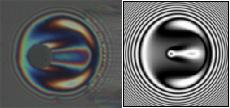
\includegraphics[width=5cm]{body/images/figure_example.png} 
	\caption{Exemple de figure avec légende}
	\label{fig:exemple}
\end{figure}

\subparagraph{Titre de niveau 5}

Isdem diebus Apollinaris Domitiani gener, paulo ante agens palatii Caesaris curam, ad Mesopotamiam missus a socero per militares numeros immodice scrutabatur, an quaedam altiora meditantis iam Galli secreta susceperint scripta, qui conpertis Antiochiae gestis per minorem Armeniam lapsus Constantinopolim petit exindeque per protectores retractus artissime tenebatur.

Titre de niveau 6
Non ergo erunt homines deliciis diffluentes audiendi,

\subsection{Savoir-faire de Data-Gest}
\paragraph{}
Data Gest se caractérise par son approche concrète et globale du marketing opérationnel.
Ses différents pôles de compétences transversales sont entièrement internalisés :\\[1em]
\begin{itemize}
  \item Pôle stratégique pour vous accompagner dans la définition, la réalisation et la mise en place de vos actions marketing.
  \item Studio création graphique et conception web : pour dynamiser vos supports de communication.
  \item Division opérationnelle pour le suivi commercial et logistique de vos campagnes.
  \item Département dotations / cadeaux d’affaires : base de données cadeaux de plusieurs milliers d'articles issus d'univers variés (maroquinerie, bricolage, high-tech, électroménager, horlogerie....).

\end{itemize}




\section{Introduction du sujet}
\justifying
\subsection{Description}
\paragraph{}
Data-Gest est une agence spécialisée dans le marketing opérationnel (programmes de fidélisation et de parrainages, challenges commerciaux'). Depuis sa création en 2000, la société est en forte croissance et travaille essentiellement avec de grand comptes ( Allianz, La Poste, Air France')
\paragraph{}


Au sein du « département Web \& nouvelles technologies » et en liaison avec le pôle Marketing et Commercial, je suis en charge du développement et de l'évolution de nos solutions Web. 
Mes missions principales :
\begin{figure}
  \centering
  \subfigure[Air france]{\label{fig:air france}
\includegraphics[width=0.3\textwidth]{body/images/air-france-logo.jpg}}                
  \subfigure[Allianz]{\label{fig:Allianz}
\includegraphics[width=0.3\textwidth]{body/images/allianz.jpeg}}
  \subfigure[La poste]{\label{fig:mouse}
\includegraphics[width=0.3\textwidth]{body/images/laposte.png}}
  \caption{Partenaire de Data-Gest}
  \label{fig:Partenaire de Data-Gest}
\end{figure}

\begin{itemize}
  \item [-]Prise de brief 
  \item [-]Rédaction des spécifications fonctionnelles et des story-boards, 
  \item [-]Contrôle qualité et test, 
  \item [-]Intégration XHTML / CSS
  \item [-]bon respect de la méthodologie projet,
  \item [-]respect des budgets et des délais, 
\end{itemize}

\subsection{Objet final}
\paragraph{}
Bien amélioration du frame-work de l'entreprise : KdoMotive
Réaliser le projet pendant le période de stage. Et corriger le bug, tester le site, et aussi améliorer les codes

\subsection{Organisation du travail}
Déroulement:

TODO: diagramme du gantt
ou table de bilan
%\input{body/pages/chapitre-intro/intro-sujet/}



\chapter{Pré études}\thispagestyle{fancy}
\paragraph{}
Avant de commencer le travail, j'ai pris 3 semaine afin de bien comprendre comment fonctionne les mécanismes de pôle web chez Data-Gest.Ci-dessous sont les parties principales.

\section{Serveur}
%\justifying

%Spécialisée dans le marketing opérationnel, DATA-GEST évolue depuis plusieurs années sur le marché de la stimulation des ventes et du cadeau d’affaires.\\[2ex]

\subsection{Serveur local}


\subsubsection{Infrastructure}
Il y a trois serveurs locals chez Data-Gest. 
\begin{description}
\item[•]DATAGESTSRV01
\item[•]DATAGESTSRV02
\item[•]SRV-NAVISION
\end{description}


\subparagraph{}
L'infrastructure est déjà configurée en mode failover. C'est à dire que l'ip sur lequel le service est hébergé est routé sur le
serveur princial (ns26393.ovh.net). En cas de panne du serveur principale l'adresse ip est routée vers le serveur
secondaire. Par conséquent il faudra configurer les domaines de production pour qu'ils dirigent vers l'adresse IP
178.33.251.180.




%\begin{itemize}
%\item Liste a puces 1
%			\begin{itemize}
%			\item Liste a puces 2
%						\begin{itemize}
%						\item Liste a puces 3
%						\end{itemize}
%			\end{itemize}
%\end{itemize} 
%
%\paragraph{Titre de niveau 4}
%Non ergo erunt homines deliciis diffluentes audiendi, si quando de amicitia, quam nec usu nec ratione habent cognitam, disputabunt.
%
%\begin{figure}[H]
%	\center
%	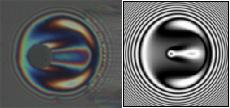
\includegraphics[width=5cm]{body/images/figure_example.png} 
%	\caption{Exemple de figure avec légende}
%	\label{fig:exemple}
%\end{figure}
%
%\subparagraph{Titre de niveau 5}
%
%Isdem diebus Apollinaris Domitiani gener, paulo ante agens palatii Caesaris curam, ad Mesopotamiam missus a socero per militares numeros immodice scrutabatur, an quaedam altiora meditantis iam Galli secreta susceperint scripta, qui conpertis Antiochiae gestis per minorem Armeniam lapsus Constantinopolim petit exindeque per protectores retractus artissime tenebatur.
%
%Titre de niveau 6
%Non ergo erunt homines deliciis diffluentes audiendi,




\subsection{Serveur distant}
\paragraph{}
Les serveurs de distants de Data-Gest sont gérés par OVH. Les services suivant sont déjà mis en place par défaut: 

%\begin{itemize}
%\item Liste a puces 1
%			\begin{itemize}
%			\item Liste a puces 2
%						\begin{itemize}
%						\item Liste a puces 3
%						\end{itemize}
%			\end{itemize}
%\end{itemize} 
%
%\paragraph{Titre de niveau 4}
%Non ergo erunt homines deliciis diffluentes audiendi, si quando de amicitia, quam nec usu nec ratione habent cognitam, disputabunt.
%
%\begin{figure}[H]
%	\center
%	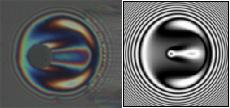
\includegraphics[width=5cm]{body/images/figure_example.png} 
%	\caption{Exemple de figure avec légende}
%	\label{fig:exemple}
%\end{figure}
%
%\subparagraph{Titre de niveau 5}
%
%Isdem diebus Apollinaris Domitiani gener, paulo ante agens palatii Caesaris curam, ad Mesopotamiam missus a socero per militares numeros immodice scrutabatur, an quaedam altiora meditantis iam Galli secreta susceperint scripta, qui conpertis Antiochiae gestis per minorem Armeniam lapsus Constantinopolim petit exindeque per protectores retractus artissime tenebatur.
%
%Titre de niveau 6
%Non ergo erunt homines deliciis diffluentes audiendi,

\subsection{Savoir-faire de Data-Gest}
\paragraph{}
Data Gest se caractérise par son approche concrète et globale du marketing opérationnel.
Ses différents pôles de compétences transversales sont entièrement internalisés :\\[1em]
\begin{itemize}
  \item Pôle stratégique pour vous accompagner dans la définition, la réalisation et la mise en place de vos actions marketing.
  \item Studio création graphique et conception web : pour dynamiser vos supports de communication.
  \item Division opérationnelle pour le suivi commercial et logistique de vos campagnes.
  \item Département dotations / cadeaux d’affaires : base de données cadeaux de plusieurs milliers d'articles issus d'univers variés (maroquinerie, bricolage, high-tech, électroménager, horlogerie....).

\end{itemize}



\section{ModuleDG}
%\justifying

\paragraph{}
ModuleDG est un web service développé par Data-Gest qui sert à :
\begin{itemize}
\item [-] Gestion des commandes envoyé depuis chaque site.
\item [-] Gestion de la base de donnée de cadeaux total. 
\item [-] Gestion de la sélection de cadeaux de chaque site.
\end{itemize}

\paragraph{}
La fonctionnalité est bien illustré dans le figure suivant.

[TODO: structure de ModuleDG et chaque site]

En fait chaque site a une sélection de cadeaux qui est géré par  ModuleDG. Quand le client de chaque site valide un commande, il sera passé à moduleDG pour le contrôler. 



\backmatter
\chapter{Conclusion}
%\addcontentsline{toc}{section}{Conclusion}

Lorsque de mon stage de fin d'étude de 6 mois, j'ai appris beaucoup de chose.

Tout d'abord, j'arrive de intégration dans une équipe rapidement. Auparavant, à cause de problème de mon niveau de langue, ça prend du temps de bien comprendre le sujet et la fonctionnalité du groupe. Par conséquence, ce n'est pas pratique de intégrer dans un groupe de développement. 

Grâce à l'augmentation de niveau de mon langue français  et aussi beaucoup de méthodologie j'ai appris pendant ma formation dans filière SRI à UTC, j'arrive de intégrer dans le développement rapidement après un mois de pré études chez Data-Gest, et aussi à l'aide de mon tuteur qui m'a expliqué la  fonctionnalité et structure de framework en détail avec patience. 

Deuxièmement, j'arrive de  mettre en pratique mes connaissances théoriques acquises durant mes études à UTC . Surtout dans la partie de l'administration de système et configuration du réseaux. Après 6 mois de m'entraîner, je peux bien maîtriser VIM, et aussi beaucoup de méthodes techniques d'utiliser BASH commandes sous Linux.

Troisième, mon niveau de programmation est augmenté. Surtout dans la programmation orienté objet. Au début, j'avais juste un concept de POO, après avoir pratiqué 6 mois pendant mon stage, ma connaissance de POO est enrichi.

Dernièrement, j'ai bien pratiqué la méthodologie de la gestion du projet. Pendant mon stage, il faut souvent travailler sur plusieurs sujet simultanément. En utilisant la méthodologie, j'arrive de coordonner des différents projets. 

Le stage fin d'étude est un excellent souvenir, il constitue désormais une expérience professionnelle valorisante et encourageante pour mon carrière future. J'ai vécu une expérience enrichissante de travail pour la suite et mes futurs emplois. 

En résumé, je trouve que ce stage a été très bénéfique. Et aussi, je tiens à exprimer ma satisfaction d'avoir pu travaillé dans de bonnes conditions matérielles et un environnement agréable



\bibliographystyle{plain}
\bibliography{biblio}\addcontentsline{toc}{chapter}{Bibliographie} 
\appendix
\chapter{Annexe}

\section{Configuration du Postfix}

\lstinputlisting[language=bash, frame=shadowbox, numbers=left, numberstyle=\tiny, stringstyle=\color{red}]{appendix/main.cf}


\end{document}
